\nxsection{Le R\^ole ''Administrateur''}\label{sec:utilisateurs-ladministrateur}
\index{administrateur}
\index{LAdministrateur}

La figure~\ref{fig:fenetre-principale-admin} illustre la
fen\^etre d'acceuil d'un utilisateur avec le \role \admin,
apr\`es qu'il se soit enregistr\'e dans \yeroth.\\

\begin{figure}[!htbp]
\centering
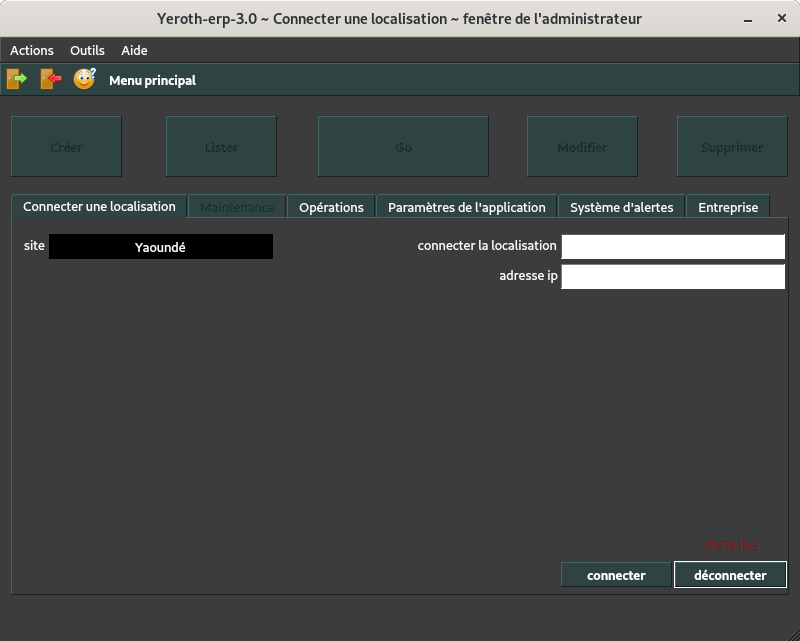
\includegraphics[scale=0.63]{images/yeroth-fenetre-administrateur.png}
\caption{La fen\^etre d'acceuil d'un \admin.}
\label{fig:fenetre-principale-admin}
\end{figure}

Un utilisateur avec le \role \admin a acc\`es aux
fonctionnalit\'es suivantes:
\begin{enumerate}[1)]
	\item arr\^eter le syst\`eme d'alerte
	\item connecter \yerothpos \`a une autre localisation
	\item d\'emarrer le syst\`eme d'alerte
	\item modifier les param\`etres de l'application
	\item modifier les param\`etres du syst\`eme d'alerte.\\   
\end{enumerate}

Un utilisateur avec le \role \admin assume les
t\^aches de cr\'eer et de maintenir les objets suivants:
\begin{enumerate}[1)]
	\item les alertes (sur une p\'eriode de temps, ou sur une quantit\'e en stock)
	%\item les bons de commande
	\item les cat\'egories d'articles
	\item les clients
	\item les comptes utilisateurs
	\item les fournisseurs				
	\item les localisations (une localisation est un site de
	      l'entreprise o\`u se trouve un ou plusieurs stocks).\\   
\end{enumerate}
